\section{Inngangur}
Skýrsla þessi fjallar um gerð á leikjatölvu sem notfærir sér Raspberry Pi 3 með RetroPie stýrikerfinu.

Með tilkomu snjallsímans er nú langflestum íslendingum kleift að spila tölvuleiki hvar sem þeir eru. Það eru þó nokkrir stórir gallar við það að spila leiki á símanum þínum. Þess vegna erum við að gera okkar eigin fartæka tölvu sem er hönnuð til þess að spila leiki. Aðalvandamálið við tölvuleiki á farsímum er að sjálfsögðu það að það eru nánast engir takkar á flestum snjallsímum í dag. Annað er það hvað flest stýrikerfi á símum eru lokuð. Það þýðir að við getum ekki bara spilað einhvern af uppáhaldsleikjunum okkar á símanum. Apple eða Google þurfa að leyfa okkur það fyrst. Verkefnið okkar er að gera ferðaleikjatölvu. Með því að nýta opna hugbúnaðarkerfi einkatölvunnar getum við opnað gáttina til fyrir það að spila alla leiki. Með því að hafa bæði takka og snertiskjá innbyggða getum við stutt alla bestu leikina, meira að segja þá sem komu út fyrir 30 árum. Með því að nota kerfi sem hefur hlotið stuðning í fjölda ára, RetroPie \cite{mckittrick2015retropie}, getum við verið viss um að þetta mun virka. Hérna á myndinni er planið okkar:

\begin{figure}[h]
\includegraphics[scale=.3]{img/Portable_RetroPie_Diagram}
\end{figure}
\section{Um verkefnið}
Við ætlum að gera ferða-leikjatölvu. Hún verður byggð á raspberry pi 3 model B og mun keyra RetroPie stýrikerfið. Hún mun geta spilað alls konar leiki frá Mario til Doom. Tölvan notar snertiskjá sem verður vonandi hægt verður að nota í leikjum (sem auka takka eða eitthvað), það verður rafhlaða, og hátalarar fyrir hljóð. Hægt verður að hlaða hana með micro-USB snúru. Til þess að gera þetta allt saman þurfum við að leysa ýmis vandamál eins og hvaða búnað það væri best að nota, samsetningu og uppsetningu á hugbúnaði. 

\subsection{Hönnun}

Áður en við getum í raun hafið verkefnið verðum við fyrst að hanna vélina. Það er því miður mjög erfitt að breyta til eftir að búið er að festa kaup á pörtum, svo við verðum að vanda okkur við valið.

Tölvan á eftir að líkjast spjaldtölvu í útliti. Tölvan á eftir að vera með innbyggða stýripinna, takka og örvatakka (directional pad), Í miðjunni verður 7 tommu snertiskjár, og það verða tveir hátalarar sem eiga eftir að beina að leikmanninum (beint fram) eða út til hliðanna, að láta hátalarana beina beint fram væri betri kosturinn, en það kemur í ljós hvort það sé nóg pláss.

Skelin utan um tölvuna á eftir að vera 3D prentuð, og verður hún nógu stór til að rúma allan vélbúnað og batterí innan henni. Ýmsir takkar eiga eftir að vera utan á tölvunni eins og takki til að slökkva og kveikja á henni, og potentiometer til að stýra hljóðstyrk

Sem dæmi um útlit sjá Nintendo Switch.

\begin{figure}[h]
	\centering
	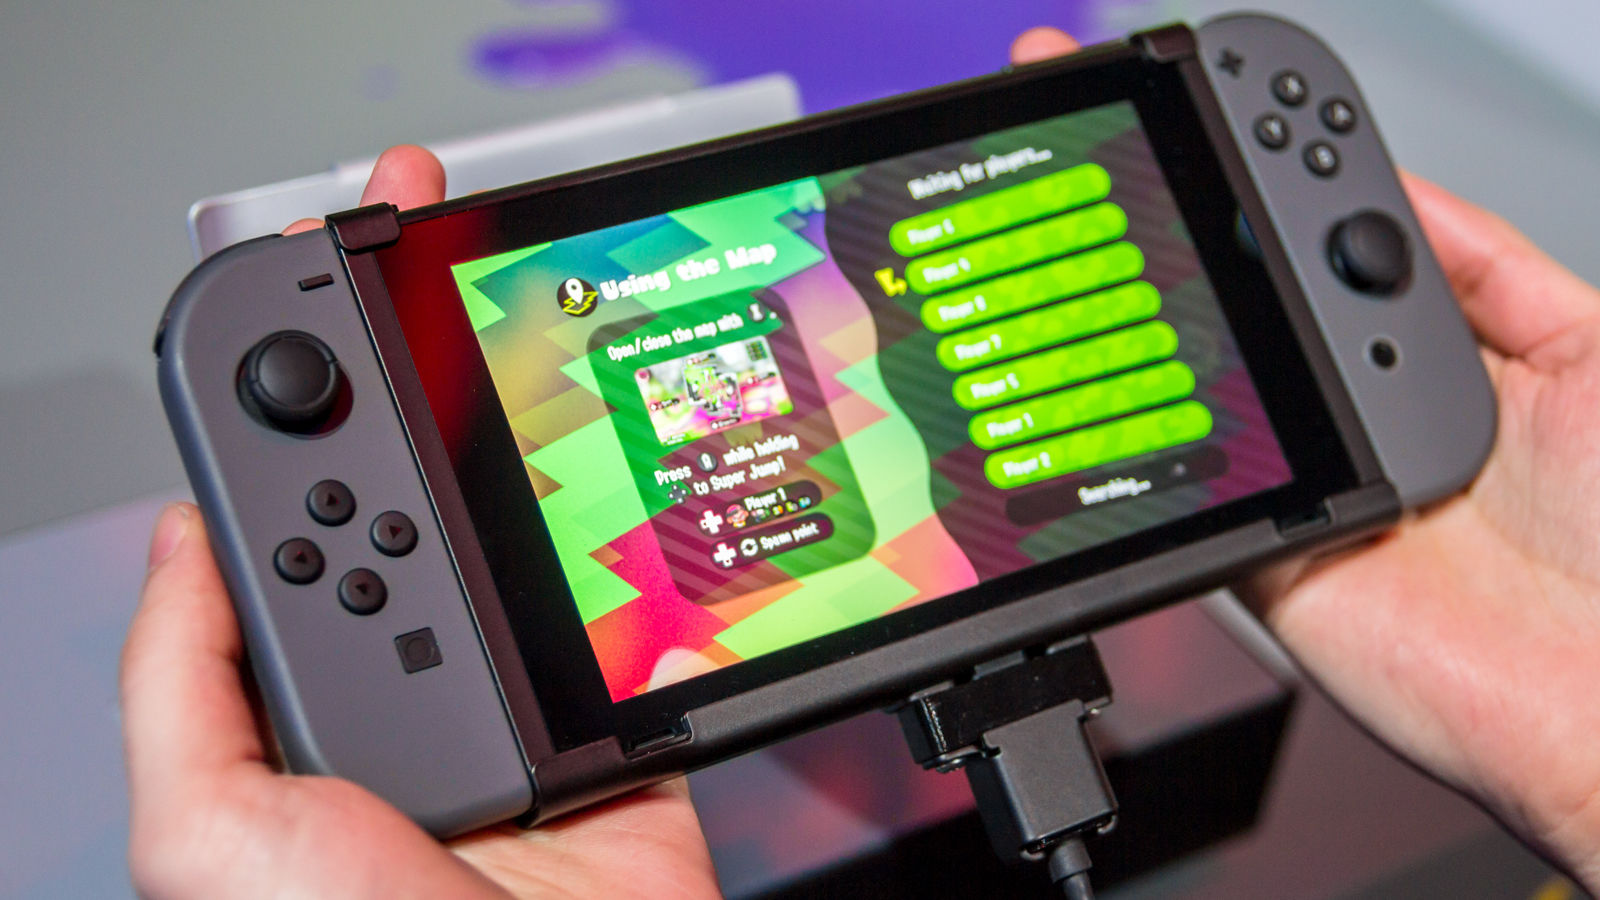
\includegraphics[scale=.5]{img/switch}
	\caption{Nintendo Switch}
\end{figure}

\subsection{Samsetning}

Eftir að við erum komnir með alla partana og hönnunin er tilbúin er samsetningin næst. Við þurfum örugglega að lóða saman víra og skrúfa saman parta. Við munum 3d-prenta skelina utan um vélina með hjálp FabLab í Breiðholtinu.

\subsection{Hugbúnaður}

Þegar við erum búnir að setja saman alla partana þurfum við að huga að hugbúnaðinum. Við ætlum að nota RetroPi stýrikerfið, sem inniheldur heilann helling af emulator-um, sem spila gamla leiki. Við þurfum að gera einhver script til að passa upp á að allt saman hagi sér rétt, við viljum að þú getir stjórnað öllu saman bara með tökkunum á unitinu, án þess að þurfa að tengja auka lyklaborð við eða eitthvað. Svo þurfum við líka að passa að takkarnir, hátalarar og skjárinn tengjast rétt við stýrikerfið.

\subsection{Af hverju þetta verkefni?}

Vegna þess að það er skemmtilegt!

Við völdum þetta verkefni af því að við höfum gaman af tölvuleikjum og okkur langaði til að gera leikjatölvu. Okkur fannst þetta spennandi hugmynd. Það að við höfum möguleikann á að gera þetta verkefni yfir höfuð er æðislegt.

\subsection{Nothæfi}

Þessa leikjatölvu væri hægt að nota í, eins og nafnið gefur til, ýmsa tölvuleiki. Það væri hægt að fjöldaframleiða og selja svona tölvur. Á markaðinum núna eru til ýmsar leikjatölvur sem spila gamla leiki, en þær spila yfirleitt bara leiki frá einu fyrirtæki og svo þarftu alltaf að tengja það við sjónvarpið. Með okkar tölvu gætir þú spilað nánast hvaða gamla leik sem er (svo lengi sem þú átt ROM-ið) og tekið þá með þér. Þetta er betra en síminn þinn því hann kemur ekki með neinum tökkum sem hægt er að nota til að stjórna leiknum, bara snertiskjá.